\section{Collision Detection}
Collision detection is a subject at the center of physics simulators. To build a simulation of the robot in its environment, the main loop goes as follows:
\begin{enumerate}
    \item Collision detection: finding contact points
    \item Collision resolution: finding contact forces using physical principles
    \item Time integration: update of the quantities of interest (position, velocity, etc.)
\end{enumerate}
It is therefore crucial to have an efficient collision detection algorithm, that is to know whether two objects are in contact or not, and if so, to find the contact points.

Nevertheless, collision detection is a computational bottleneck in physics simulators. Resolving collision detection for one pair of objects takes a significant amount of time, especially for complex shapes, and the number of pairs to check grows quadratically with the number of objects. A general method to optimize such a process is to decompose one collision detection into two phases, the broad phase and the narrow phase. The broad phase uses simple geometric primitives to quickly discard pairs of objects that are far from colliding. The narrow phase then uses more complex geometric primitives to find the exact contact points.

\subsection{The broad phase}
\subsubsection{Bounding volumes}
As described previously, the broad phase uses \emph{bounding volumes} (BVs) to prune collisions: we will only check the overlapping BVs, and leave fine-grain detection for the narrow phase. The main goal is to efficiently determine when two objects are far from overlapping, to prune such pairs of objects. Therefore, we will always use an over-approximation of the shape of the object, but never an under-approximation. We accept to mark as a likely collision two objects that are not intersecting, but we do not want to miss any. 

The narrow phase will later determine which pairs are actually colliding, and which aren't, using exact representation of the objects. This two-phases approach allows for improved performance without sacrificing the precision of the detector.

\subsubsection{Example of bounding volumes}
The choice of a bounding volume is always a tradeoff between performance and precision. Larger BVs such as spheres or axis-aligned bounding boxes rely on extremly efficient algorithms, at the cost of a poor representation of the actual volume of the object. On the other hand, complex volumes such as the convex hull represent precisely the objects while requiring a longer time to compute collisions.
\begin{figure}[H]
    \centering
    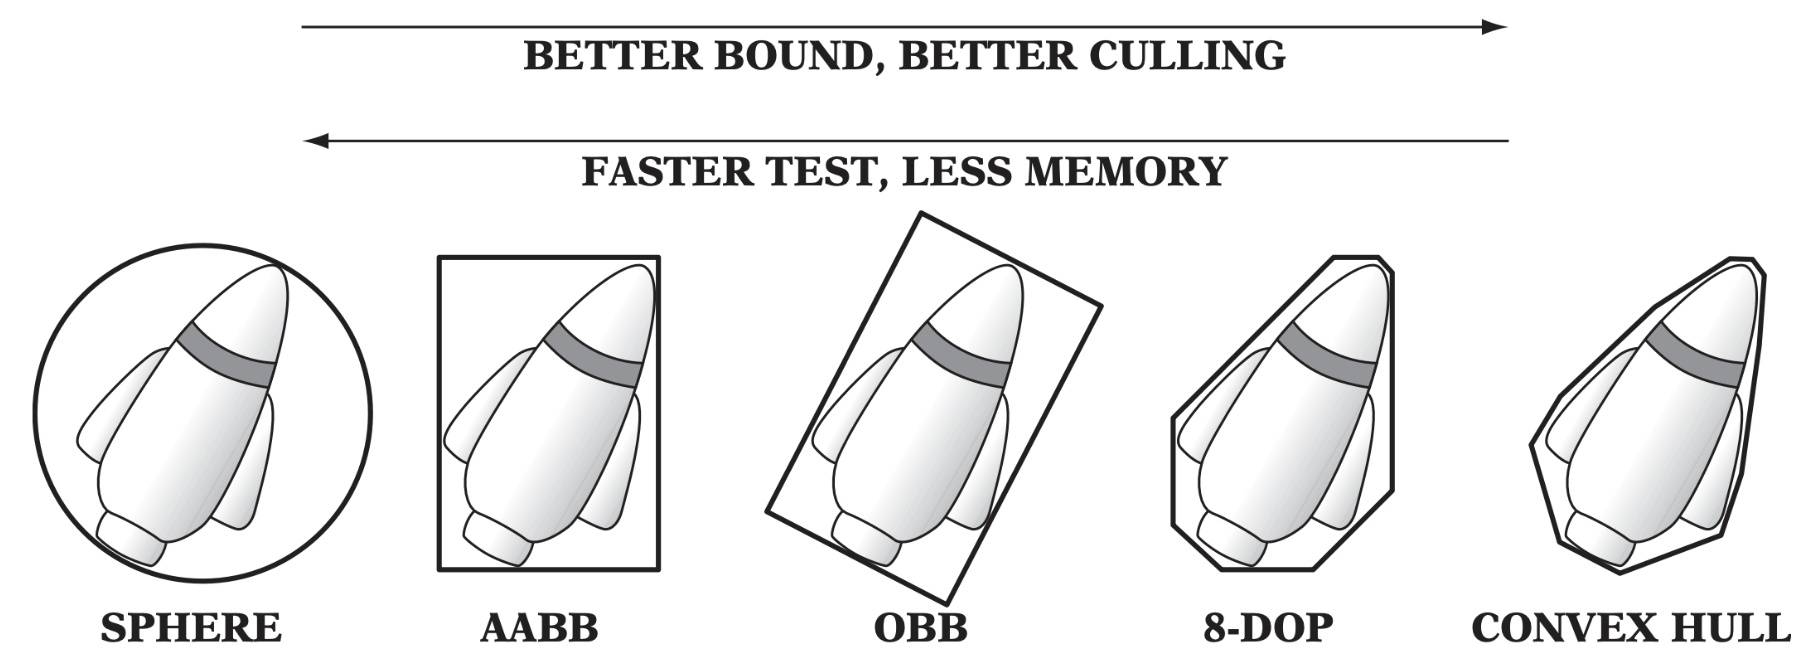
\includegraphics[width=.7\textwidth]{collision-detection/bv-examples.png}
    \caption{Examples of bounding volumes.}
\end{figure}
It is worth noting two important examples: Axis-Aligned Bounding Boxes (AABB) and Oriented Bounding Boxes (OBB), which can be efficiently computed, and represent accurately most objects we might have to deal with. Note that the choice of the axes is arbitrary.

\subsubsection{Dynamic tree representation}
Given any representation of the bounding volumes of the objects of the scene, an efficient way to compute the potential collisions between these objects is to build a \emph{dynamic tree}.
\begin{figure}[H]
    \centering
    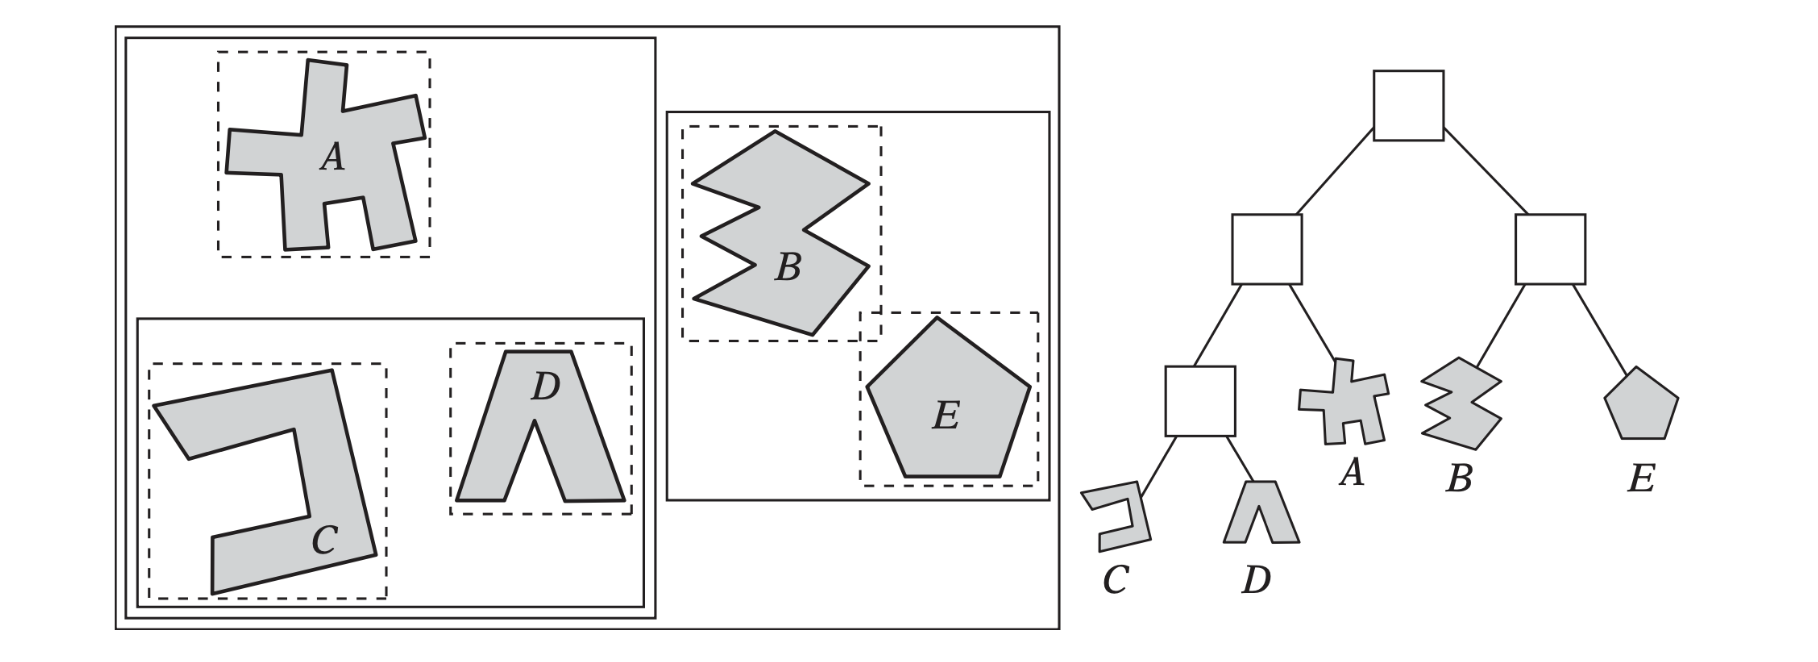
\includegraphics[width=.8\textwidth]{collision-detection/tree.png}
\end{figure}
The idea is to split the scene into primitives that are easy to compute, for instance AABBs, such that any object is in exactly one subpart of the scene. Therefore, two objects are coliding only if they are children of the same node of the tree, which drastically reduces the number of collisions to check.

\subsubsection{Sweep and Prune algorithm}
When using exclusively AABBs, another efficient approach is to use the \emph{Sweep and Prune} (SaP) algorithm. Its idea is to sort the bounding boxes along each axis of their axis. Objects may overlap at their starts or ends; if two objects are overlapping for every axis, one can conclude that their AABBs collide.
\begin{figure}[H]
    \centering
    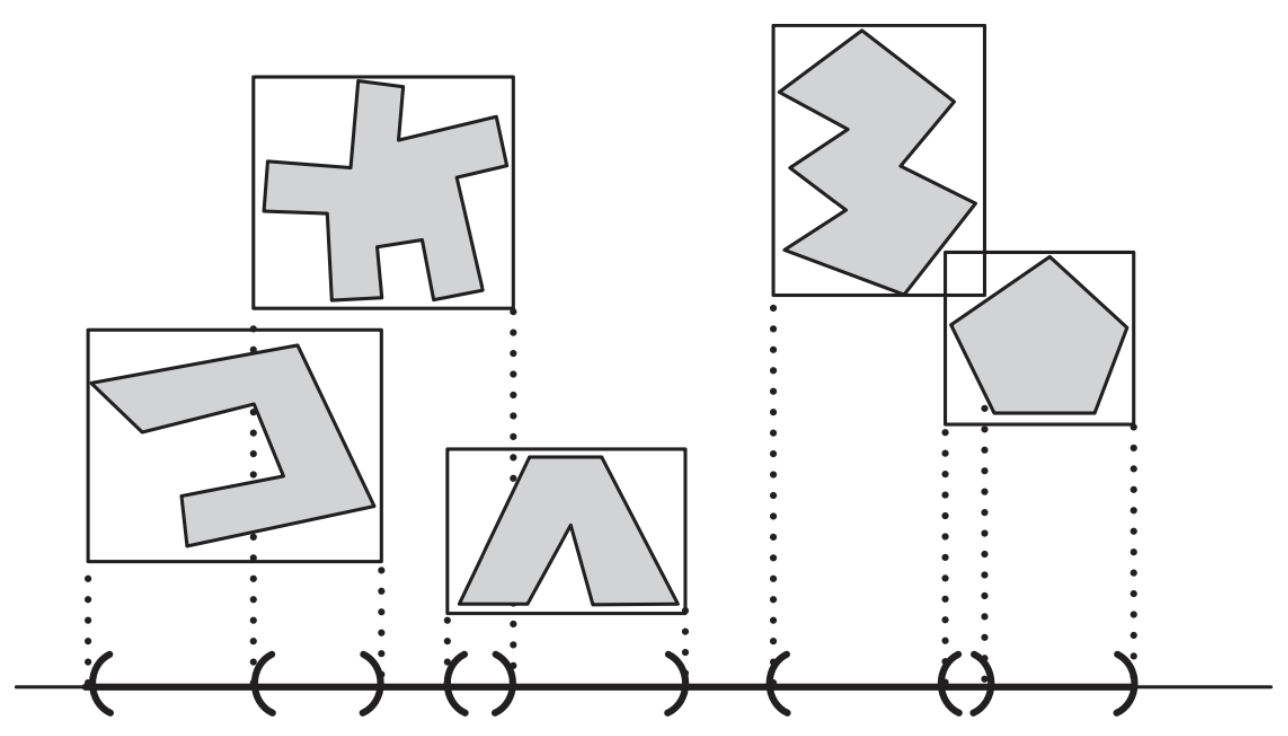
\includegraphics[width=.5\textwidth]{collision-detection/sap.png}
\end{figure}
Such a method can become problematic if multiple objects are almost aligned on the same line.
\begin{figure}[H]
    \centering
    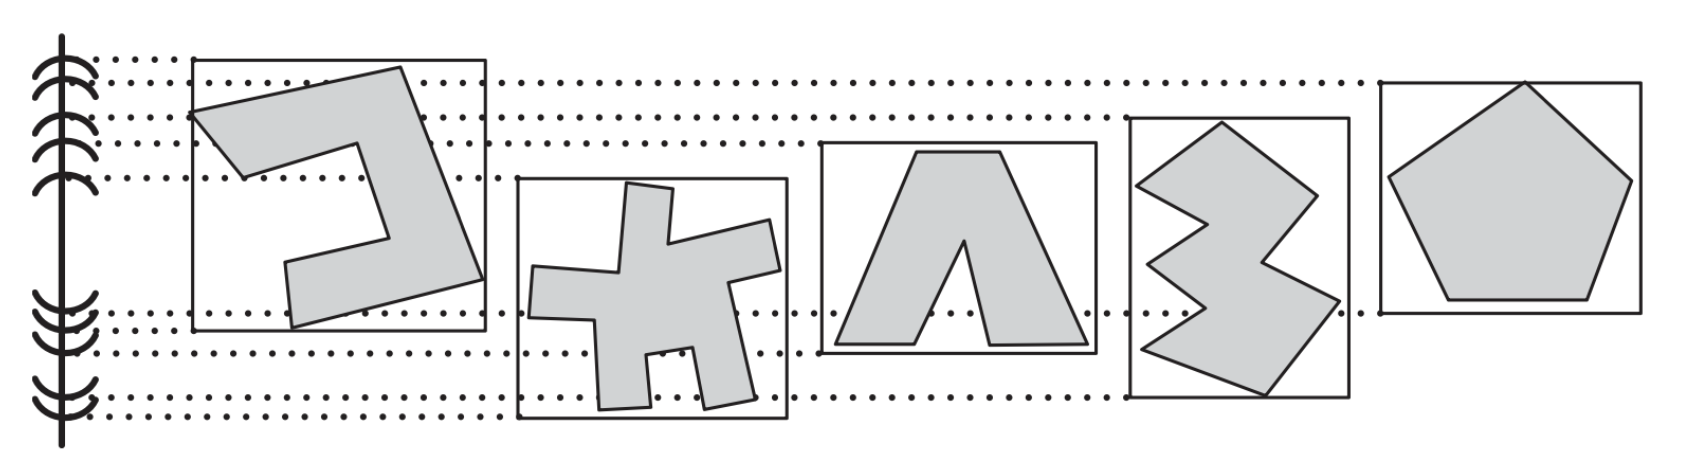
\includegraphics[width=.8\textwidth]{collision-detection/sap-aligned.png}
\end{figure}

\subsection{The narrow phase}

\newpage